
% Spellcheck: ok
% Mikes: none

\chapter{Predictive Analytics}{}{}
\label{ch:prediction}

\index{data analysis!predictive analytics|(} 
\index{predictive analytics|(} 

% ============================================================
%\section{Introduction}

\index{predictive analytics!about|(}
 
\Fint{Data analysis can take many different forms---not only in the
techniques that we apply but also} in the \emph{kind} of results that
we ultimately achieve. Looking back over the material that we have
covered so far, we see that the results obtained in Part
\ref{part:graphics} were mostly \emph{descriptive}: we tried to figure
out what the data was telling us and to describe it. In contrast, the
results in Part \ref{part:analytics} were primarily
\emph{prescriptive}: data was used as a guide for building models
which could then be used to infer or prescribe phenomena, including
effects that had not actually been observed yet.  In this form of
analysis, data is not used directly; instead it is used only
indirectly to guide (and verify) our intuition when building models.
Additionally, as I tried to stress in those chapters, we don't just
follow data blindly, but instead we try to develop an understanding of
the processes that generate the data and to capture this understanding
in the models we develop. The predictive power of such models derives
from this \emph{understanding} we develop by studying data and the
circumstances in which it is generated.\footnote{The techniques
  discussed in Part \ref{part:computation} are different: for the most
  part they were strictly computational and can be applied to any
  purpose, depending on the context.}

In this chapter, we consider yet another way to use data---we can call
it \emph{predictive}, since the purpose will be to make predictions
about future events. What is different is that now we try to make
predictions \emph{directly from the data} without necessarily forming
the kind of conceptual model (and the associated deeper understanding
of the problem domain) as discussed in Part \ref{part:analytics}.
This difference is obviously both a strength and a  weakness. It's a
strength in that it enables us to deal with problems for which we have
no hope of developing a conceptual model, given the complexity of the
situation. It is also a weakness because we may end up with only a
black-box solution\vadjust{\pagebreak} and no deeper understanding.  There are technical
difficulties also: this form of analysis tends to require huge 
data sets because we are lacking the consistency and continuity
guarantees provided by a conceptual model. (We will come back to this
point.)

\section{Topics in Predictive Analytics}

The phrase \emph{predictive analytics} is a bit of an umbrella term
(others might say: marketing term) for various tasks that share the
intent of deriving predictive information directly from data. Three
different specific application areas stand out:
\begin{unnumlist}
\subparagraph{Classification or supervised learning}
\index{classification!about}
\index{supervised learning} 
\item Assign each record to
  exactly one of a set of predefined classes. For example, classify
  credit card transactions as ``valid'' or ``fraudulent.'' Spam
  filtering is another example. Classification is considered
  ``supervised,'' because the classes are known ahead of time and
  don't need to be inferred from the data.  Algorithms are judged on
  their ability to assign records to the correct class.
\subparagraph{Clustering or unsupervised learning} \index{clustering!about} \index{unsupervised learning}
\item Group records into
  clusters, where the size and shape---and often even the number---of
  clusters is unknown. Clustering is considered ``unsupervised,''
  because no information about the clusters is available ahead of the
  clustering procedure.
\subparagraph{Recommendation} \index{recommendations} 
\item Recommend a suitable item based on past
  interest or behavior. Recommendation can be seen as a form of
  clustering, where you start with an anchor and then try to find
  items that are similar or related to it.
\end{unnumlist}

A fourth topic that is sometimes included is time-series forecasting.
However, I find that it~does not share many characteristics with the
other three, so I usually don't consider it part~of predictive
analytics itself. (We discussed time-series analysis and forecasting
in Chapter~\ref{ch:timeseries}.)

Of the three application areas, classification is arguably the most
important and the best developed; the rest of this chapter will try to
give an overview over the most important classification algorithms and
techniques. We discussed unsupervised learning in Chapter
\ref{ch:clustering} on clustering techniques---and I'll repeat my
impression that clustering is more an exploratory than a predictive
technique.  Recommendations are the youngest branch of predictive
analytics and quite different from the other two. (There are at least
two major differences. First, on the technical side, many
recommendation techniques boil down to network or graph algorithms,
which have little in common with the statistical techniques used for
classification and clustering. Second, recommendations tend to be
\emph{explicitly} about predicting human behavior; this poses
additional difficulties not shared by systems that follow strictly
deterministic laws.) For these reasons, I won't have much to say about
recommendation techniques here.

Let me emphasize that this chapter can serve only as an overview of
classification. Entire books could (and have!) been written about it.
But we can outline the problem, introduce some terminology, and give 
the flavor of different solution approaches.

\index{predictive analytics!about|)}

\leaflong{-13pt}

% ============================================================
\section{Some Classification Terminology}

\index{predictive analytics!classification terminology} 
\index{classification!terminology!}
 
We begin with a data set containing multiple elements, records, or
\emph{instances}.  Each instance consists of several \emph{attributes}
or \emph{features}.  One of the features is special: it denotes the
record's \emph{class} and is known as the \emph{class label}. Each
record belongs to exactly one class.

A large number of classification problems are binary, consisting only
of two classes (valid or fraudulent, spam or not spam); however,
multiclass scenarios do also occur. Many classification algorithms can
deal only with binary problems, but this is not a real limitation
because any multiclass problem can be treated as a \emph{set} of
binary problems (belongs to the target class or does belong to any
other class).

A \emph{classifier} takes a record (\ie, a set of attribute values)
and produces a class label for this record. Building and using a
classifier generally follows a three-step process of training,
testing, and actual application.

We first split the existing data set into a \emph{training set} \index{training sets} and a
\emph{test set}. \index{test sets} In the training phase, we present each record from
the training set to the classification algorithm. Next we compare the
class label produced by the algorithm to the true class label of the
record in question; then we adjust the algorithm's ``parameters'' to
achieve the greatest possible accuracy or, equivalently, the lowest
possible error rate. (Of course, the details of this ``fitting''
process vary greatly from one algorithm to the next; we will look at
different ways of how this is done in the next section.)

The results can be summarized in a so-called \emph{confusion matrix} \index{confusion matrices} 
whose entries are the number of records in each category. (Table
\ref{tbl:confusion} shows the layout of a generic confusion matrix.)

\begin{table}
\def\vrl{\smash{\vrule height38.7pt width.25pt depth3pt}}%
\tbl{The confusion matrix for a binary classification problem\label{tbl:confusion}}{%
\tabcolsep11pt\begin{tabular}{lcccc}
\toprule
            && \TCH{Predicted: A} && \TCH{Predicted: B} \\
 \colrule 
\TCH{Actual: A}  && Correct      && Incorrect \\\colrule 
\TCH{Actual: B}   &\vrl& Incorrect   &\vrl & Correct \\
\end{tabular}}
\end{table}

Unfortunately, the error rate derived from the training set (the
\emph{training error}) is typically way too optimistic as an indicator
of the error rate the classifier would achieve on new data---that is,
on data that was not used during the learning phase.  This is the
purpose of  the~test set: after we have optimized the algorithm using
\emph{only} the training data, we let the classifier operate on the
elements of the test set to see how well it classifies them.  The
error rate obtained in this way is the \emph{generalization error} \index{generalization errors} and
is a much more reliable indicator of the accuracy of the classifier.

To understand the need for a separate testing phase (using a separate
data set!), keep in mind that as long as we use enough parameters
(\ie, making the classifier more and more complex) we can always tweak
a classifier until it works very well on the training set. But in
doing so, we train the classifier to memorize every aspect of the
training set, including those that are atypical for the system in
general. We therefore need to find the right level of complexity for
the classifier. On the one hand, if it is too simple, then it cannot
represent the desired behavior very well, and both its training and
generalization error will be poor; this is known as
\emph{underfitting}. \index{underfitting} On the other hand, if we make the classifier too
complex, then it will perform very well on the training set (low
training error) but will not generalize well to unknown data points
(high generalization error); this is known as \emph{overfitting}. \index{overfitting} 
Figure \ref{fig:overfitting} summarizes these concepts.

\begin{figure}
\centerline{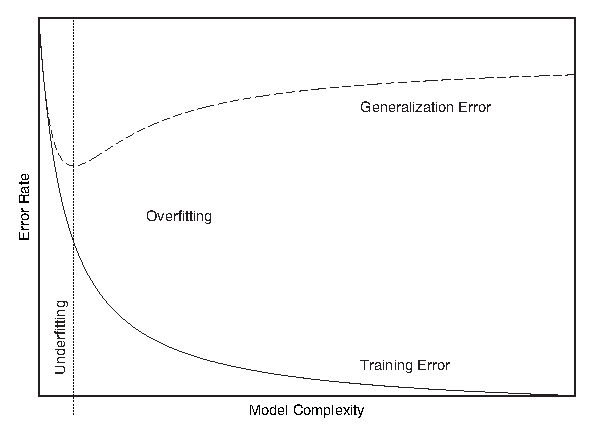
\includegraphics{img/overfitting}}
  \caption{Overfitting: as a model becomes more complex, it becomes
    increasingly able to represent the \emph{training} data. However,
    such a model is overfitted and will not generalize well to data
    that was not used during training.}
  \label{fig:overfitting}%\vspace*{-8pt}
\end{figure}

Once a classifier has been developed and tested, it can be used to
classify truly new and unknown data points---that is, data points for
which the correct class label is not known. (This is in contrast to
the test set, where the class labels were known but not used by the
classifier when making a prediction.)\vspace*{-4pt}


% ============================================================
\section{Algorithms for Classification}

\index{predictive analytics!algorithms for classification|(}
\index{algorithms, for classification|(}
  
At least half a dozen different families of classification algorithms
have been developed. In this section, we briefly characterize the
basic idea underlying each algorithm, emphasizing how it differs from
competing methods. The first two algorithms (nearest-neighbor and
Bayesian classifiers) are simpler, both technically and conceptually,
than\vadjust{\pagebreak} the other; I discuss them in more detail since you may want to
implement them yourself. For the other algorithms, you probably want
to use existing libraries instead!


\subsection{Instance-Based Classifiers and Nearest-Neighbor Methods}

\index{instance-based classifiers} 
\index{nearest-neighbor methods} 

The idea behind instance-based classifiers is dead simple: to classify
an unknown instance, find an existing instance that is ``most similar''
to the new instance and assign the class label of the known instance
to the new one!

This basic idea can be generalized in a variety of ways. First of all,
the notion of ``most similar'' brings us back to the notion of
distance and similarity measures introduced in Chapter
\ref{ch:clustering}; obviously we have considerable flexibility in the
choice of which distance measure to use. Furthermore, we don't have to
stop at a single ``most similar'' existing instance.  We might instead
take the nearest $k$ neighbors and use them to classify the new
instance, typically by using a majority rule (\ie, we assign the new
instance to the class that occurs most often among the $k$ neighbors).
We could even employ a weighted-majority rule whereby ``more similar''
neighbors contribute more strongly than those farther away.

Instance-based classifiers are atypical in that they don't have a
separate ``training'' phase; for this reason, they are also known as
``lazy learners.'' (The only adjustable parameter is the extent $k$ of
the neighborhood used for classification.)  However, a (possibly
large) set of known instances must be kept available during the final
application phase.  For the same reason, classification can be
relatively expensive because the set of existing instances must be
searched for appropriate neighbors.

Instance-based classifiers are \emph{local}: they do not take the 
overall distribution of points into account. Additionally, they 
impose no particular shape or geometry on the decision boundaries
that they generate. In this sense they are especially flexible.
On the other hand, the are also susceptible to noise. 

Finally, instance-based classifiers depend on the proper choice of
distance measure, much as clustering algorithms do. We encountered
this situation before, when we discussed the need for scale
normalization in Chapters \ref{ch:clustering} and \ref{ch:reduction};
the same considerations apply here as well.

\subsection{Bayesian Classifiers}

\index{Bayesian classifiers|(} 

A Bayesian classifier takes a probabilistic (\ie,
nondeterministic) view of classification. Given a set of attributes,
it calculates the \emph{probability} of the instance to belong to
this or that class. An instance is then assigned the class label with
the highest probability.

A Bayesian classifier calculates a \emph{conditional} probability.
This is the probability of the instance to belong to a specific class
$C$, \emph{given} the set of attribute values:
%
\[
P( \text{class $C$} | \braces{x_1, x_2, x_3, \dots, x_n} )
\]
%
Here $C$ is the class label, and the set of attribute values is
$\braces{x_1, x_2, x_3, \dots, x_n}$. Note that we don't yet know the
value of the probability---if we did, we'd be finished.

To make progress, we invoke Bayes' theorem (hence the name of the
classifier---see also Chapter \ref{ch:statistics} for a discussion
of Bayes' theorem) to invert this probability expression as follows:
%
\[
P( \text{class $C$} \, | \braces{x_i} )
= \frac{ P( \braces{x_i} | \, \text{class $C$} ) 
         \cdot P( \text{class $C$} ) }
       { P( \braces{x_i} ) }
\]
%
where I have collapsed the set of $n$ features into $\braces{x_i}$ for
brevity.

The first term in the numerator (the likelihood) is the probability of
observing a set of features $\braces{x_i}$ \emph{if} the instance
belongs to class $C$ (in the language of conditional probability:
\emph{given} the class label $C$).  We can find an empirical value for
this probability from the set of training instances: it is simply the
frequency with which we observe the set of specific attribute values
$\braces{x_i}$ among instances belonging to class $C$. Empirically, we
can approximate this distribution by a set of \emph{histograms} of the
$\braces{x_i}$, one for each class label.  The second term in the
numerator, $P(\text{class $C$} )$, is the prior probability of any
instance belonging to class $C$. We can estimate this probability from
the fraction of instances in the training set that belong to class
$C$.  The denominator does not depend on the class label and---as
usual with Bayesian computations---is ignored until the end, when the
probabilities are normalized.

Through the use of Bayes' theorem, we have been able to express the
probability for an instance to belong to class $C$, given a set of
features, entirely through expressions that can be determined from the
training set.

At least in theory. In practice, it will be almost impossible to
evaluate this probability directly. Look closely at the expression
(now written again in its long form), $P( \braces{x_1, x_2, x_3,
  \dots, x_n} | \, \text{class $C$} )$. For each possible combination
of attribute values, we must have enough examples in our training set
to be able to evaluate their frequency with some degree of
reliability. This is a combinatorial nightmare! Assume that each
feature is binary (\ie, it can take on one of only two values). The
number of possible combinations is then $2^n$, so for $n=5$ we already
have $32$ different combinations. Let's say we need about 20 example
instances for each possible combination in order to evaluate the
frequency, then we'll need a training set of at least 600 instances.
In practice, the problem tends to be worse because features frequently
can take more than two values, the number of features can easily be
larger than five, and---most importantly---some combinations of
features occur much less frequently than others. We therefore need a
training set large enough to guarantee that even the least-frequent
attribute combination occurs sufficiently often.

In short, the ``brute force'' approach of evaluating the likelihood
function for all possible feature combinations is not feasible for
problems of realistic size. Instead, one uses one of two simplifications.

The \emph{naive Bayesian classifier} \index{naive Bayesian classifier} assumes that all features are
independent of each other, so that we can write:
%
\[
P( \braces{x_1, x_2, x_3, \dots, x_n} | C )
=
P( x_1 | C ) P( x_2 | C ) P( x_3 | C ) \dotsb P( x_n | C ) 
\]

This simplifies the problem greatly, because now we need only
determine the frequencies for each attribute value for a \emph{single}
attribute at a time. In other words, each probability distribution
$P(x_i|C)$ is given as the histogram of a single feature $x_i$,
separately for each class label.  Despite their simplicity, naive
Bayesian classifiers are often surprisingly effective. (Many spam
filters work this way.)

Another idea is to use a \emph{Bayesian network}. \index{Bayesian networks} Here we prune the
set of all possible feature combinations by retaining only those that
have a causal relationship with each other.

Bayesian networks are best discussed through an example. Suppose we
want to build a classifier that predicts whether we will be late to
work in the morning, based on three binary features:

\begin{itemize}
\item Alarm clock went off: Yes or No
\item Left the house on time: Yes or No
\item Traffic was bad: Yes or No
\end{itemize}

Although we don't assume that \emph{all} features are independent (as
we did for the naive Bayesian classifier), we do observe
that the traffic situation is independent of the other two features.
Furthermore, whether we leave the house on time does depend on the
proper working of the alarm clock. In other words, we can split the
full probability:
%
\[
P( \text{Arrive on time } | 
   \text{ Alarm clock, Leave on time, Traffic} )
\]
%
into the following combination of events:
\begin{gather*}
P( \text{Arrive on time } | \text{ Leave on time} ) \\
P( \text{Leave on time } | \text{ Alarm clock} ) \\
P( \text{Arrive on time } | \text{ Traffic} )
\end{gather*}

Notice that only two of the terms give the probability for the class
label (``Arrive on time'') and that one gives the probability of an
intermediate event (see Figure \ref{fig:bayesnets}).

\begin{figure}
\centerline{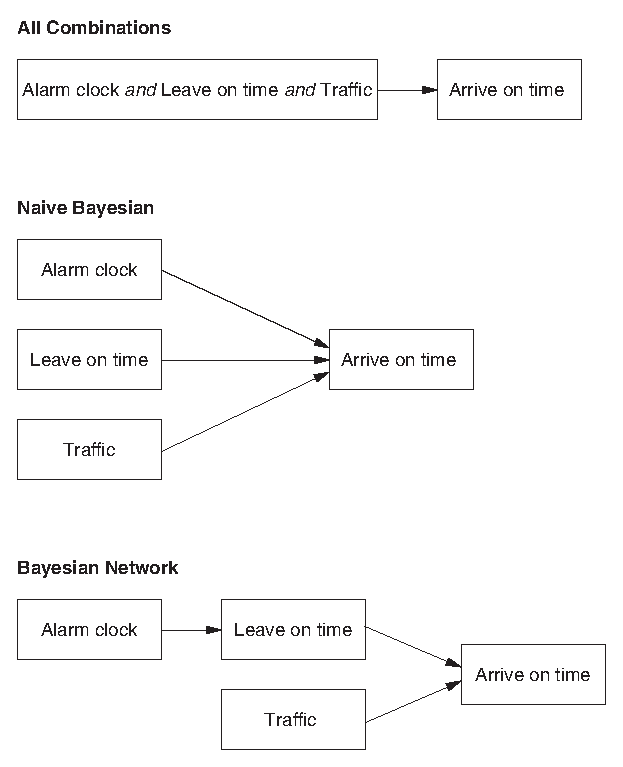
\includegraphics[scale=0.9]{img/bayesnets}}
  \caption{The structure of different Bayesian classifiers.}
  \label{fig:bayesnets}\vspace*{-9pt}
\end{figure}

For such a small example (containing only three features), the savings
compared with maintaining all feature combinations are not impressive.
But since the number of combinations grows exponentially with the
number of features, restricting our attention to only those factors
that have a causal relationship with each other can significantly
reduce the number of combinations we need to retain for larger
problems.

The structure (or \emph{topology}) \index{topology, Bayesian networks} of a Bayesian network is usually
not inferred from the data; instead, we use domain knowledge\vadjust{\pagebreak} to
determine which pathways to keep. This is exactly what we did in the
example: we ``knew'' that traffic conditions were independent of the
situation at home and used this knowledge to prune the network
accordingly.

There are some practical issues that need to be addressed when
building Bayesian classifiers. The description given here silently
assumes that all attributes are categorical (\ie, take on only a
discrete set of values). Attributes that take on continuous numerical
values either need to be discretized, or we need to find the
probability $P( \braces{x_i} | C )$ through a kernel density estimate
(see Chapter \ref{ch:univariate}) for all the points in class $C$ in
the training set. If the training set is large, the latter process may
be\vadjust{\vspace*{36pt}\pagebreak} expensive.

Another tricky detail concerns attribute values that do not occur in
the training set: the corresponding probability is $0$. But a naive
Bayesian classifier consists of a product of probabilities and
therefore becomes $0$ as soon as a single term is $0$! In particular
with small training sets, this is a problem to watch out for. On the
other hand, naive Bayesian classifiers are robust with regard to
\emph{missing} features: when information about an attribute value is
unknown for some of the instances, the corresponding probability
simply evaluates to $1$ and does not affect the final result.

\index{Bayesian classifiers|)} 

\subsection{Regression}

\index{regression!using for classification} 

Sometimes we have reason to believe that there is a functional
relationship between the class label and the set of features.  For
example, we might assume that there is some relationship between an
employee's salary and his status (employee or manager). See Figure
\ref{fig:predictregression}.

\begin{figure}
\centerline{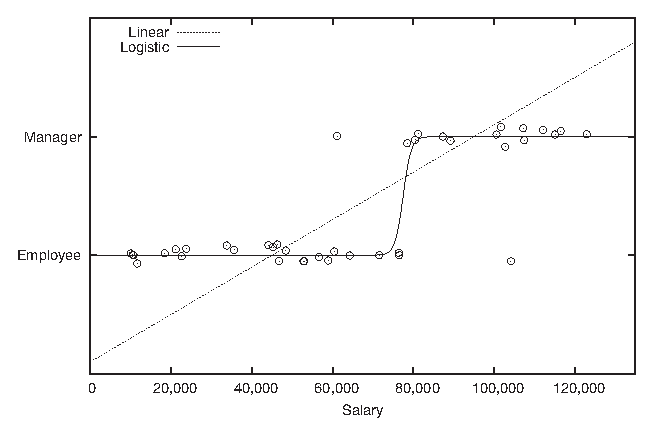
\includegraphics{img/predictregr}}
  \caption{Using regression for classification: the data points show
    the they employee type (employee or manager) as a function of the
    salary; managers tend to have higher salaries. (Data points are
    jittered in the vertical direction to avoid overplotting.)}
  \label{fig:predictregression}
\end{figure}

If it is reasonable to assume a functional relationship, then we can
try to build a classifier based on this relationship by ``fitting'' an
appropriate function to the data. This turns the classification
problem into a \emph{regression} problem.

However, as we can see in Figure \ref{fig:predictregression}, a linear
function is usually not very appropriate because it takes on all
values, whereas class labels are discrete. Instead of fitting a
straight line, we need something like a step function: a function that
is $0$ for points belonging to the one class, and $1$ for points
belonging\vadjust{\pagebreak} to the other class. Because of its discontinuity, the step
function is hard to work with; hence one typically uses the logistic
function (see Appendix \ref{app:calculus}) as a smooth approximation
to the step function.  The logistic function gives this technique its
name: \emph{logistic regression}. Like all regression methods, it is a
global technique that tries to optimize a fit over all points and not
just over a particularly relevant subset.

Logistic regression is not only important in practical applications
but has deep roots in theoretical statistics as well. Until the
arrival of support vector machines, it was the method of choice for
many classification problems.\vspace*{-4pt}


\subsection{Support Vector Machines}

\index{Support vector machines} 

Support vector machines are a relative newcomer among classification
methods. The name is a bit unfortunate: there is nothing particularly
``machine-y'' about them. They are, in fact, based on a simple
geometrical construction.

Consider training instances in a two-dimensional feature space like
the one in Figure \ref{fig:svm}. Now we are looking for the ``best''
dividing line (or \emph{decision boundary}) \index{decision boundaries} that separates instances
belonging to one class from instances belonging to the other.



We need to decide what we mean by ``best.''  The answer given by
support vector machines is that the ``best'' dividing line is one that
has the largest \emph{margin}. The margin is the space, parallel to
the decision boundary, that is free of any training instances.  Figure
\ref{fig:svm} shows two possible decision boundaries and their
respective margins. Although this example is only two-dimensional, the
reasoning generalizes directly to higher dimensions. In such cases,
the decision boundary becomes a hyperplane, and support vector
machines therefore find the \emph{maximum margin hyperplanes} \index{maximum margin hyperplanes} (a term
you might find in the literature).

I will not go through the geometry and algebra required to construct a
decision boundary from a data set, since you probably don't want to
implement it yourself, anyway. (The construction is not difficult, and
if you have some background in analytic geometry, you will be able to
do it yourself or look it up elsewhere.) The important insight is that
support vector machines turn the task of finding a decision boundary
first into the geometric task of constructing a line (or hyperplane)
from a set of points (this is an elementary task in analytic
geometry).  The next step---find the decision boundary with the
largest margin---is then just a multi-dimensional optimization
problem, with a particularly simple and well-behaved objective
function (namely, the square of the distance of each point from the
decision boundary), for which good numerical algorithms exist.

\leaflong{6pt}

One important property of support vector machines is that they perform
a strict global optimization without having to rely on heuristics.
Because of the nature of the objective function, the algorithm is
guaranteed to find the global optimum, not merely a local one. On the
other hand, the final solution does not depend on all points; instead
it depends only on those closest to the decision boundary, points that
lie right on the edge of the margin. (These are the \emph{support
  vectors}, see Figure \ref{fig:svm}.) This means\vadjust{\pagebreak} that the decision
boundary depends only on instances close to it and is not influenced
by system behavior far from the decision boundary. However, the global
nature of the algorithm implies that, for those support vectors, the
optimal hyperplane will be found!

\begin{figure}
\centerline{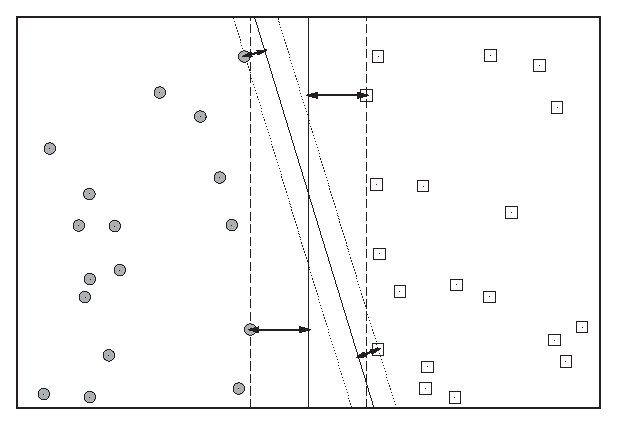
\includegraphics{img/svm}}
  \caption{Two decision boundaries and their margins. Note that the
    vertical decision boundary has a wider margin than the other one.
    The arrows indicate the distance between the respective support
    vectors and the decision boundary.}
  \label{fig:svm}\vspace*{-9pt}
\end{figure} 

Two generalizations of this basic concept are of great practical
importance. First, consider Figure \ref{fig:svm} again. We were lucky
that we could find a straight line (in fact, more than one) to
separate the data points exactly into two classes, so that both
decision boundaries shown have zero training error.  In practice, it
is not guaranteed that we will always find such a decision boundary,
and there may be some stray instances that cannot be classified
correctly by any straight-line decision boundary. More generally, it
may be advantageous to have a few misclassified training
instances---in return for a much wider margin---\break because it is
reasonable to assume that a larger margin will lead to a lower
generalization error later on. In other words, we want to find a
balance between low training error and large margin size.  This can be
done by introducing \emph{slack variables}.  Basically, they associate
a cost with each misclassified instance, and we then try to solve the
extended optimization problem, in which we try to minimize the cost of
misclassified instances while at the same time trying to maximize the
margins.

The other important generalization allows us to use curves other than
straight lines as decision boundaries. This is usually achieved
through \emph{kernelization} \index{kernelization} or the ``kernel trick.'' The basic idea
is that we can replace the dot product between two vectors (which is
central to the geometric construction required to find the maximum
margin hyperplane) with a more general function of the two vectors. As
long as this function meets certain requirements (you may find
references to ``Mercer's theorem'' in  the literature), it can be shown
that all the previous arguments continue to hold.

One disadvantage of support vector machines is that they lead to
especially opaque results: they truly are black boxes. The final
classifier may work well in practice, but it does not shed much light
on the nature of the problem. This is in contrast to techniques such
as regression or decision trees (see the next section), which often
lead to results that can be interpreted in some form.  (In regression
problems, for instance, one can often see which attributes are the
most influential ones, and which are less relevant.) 


\subsection{Decision Trees and Rule-Based Classifiers}

\index{decision trees|(}
\index{rule-based classifiers|(}  

Decision trees and rule-based classifiers are different from the
classifiers discussed so far in that they do not require a distance
measure. For this reason, they are sometimes referred to as
\emph{nonmetric classifiers}. \index{nonmetric classifiers} 

Decision trees consist of a hierarchy of decision points (the nodes of
the tree). When using a decision tree to  classify an unknown
instance, a single feature is examined at each node of the tree. Based
on the value of that feature, the next node is selected. Leaf nodes on
the tree correspond to classes; once we have reached a leaf node, the
instance in question is assigned the corresponding class label.
Figure \ref{fig:decisiontree} shows an example of a simple decision
tree.

 

The primary algorithm (\emph{Hunt's algorithm}) \index{Hunt's algorithm} for deriving a
decision tree from a training set employs a greedy approach. The
algorithm is easiest to describe when all features are categorical and
can take only one of two values (binary attributes). If this is the
case, then the algorithm proceeds as follows:
\begin{enumerate}
\item For each instance in the training set, examine each feature in
  turn. 
\item Split the training instances into two subsets based on the
  value of the current feature. 
\item Select the feature that results in the ``purest'' subsets; the
  value of this attribute will be the decision condition employed by
  the current node.
\item Repeat this algorithm recursively on the two subsets until the
  resulting subsets are sufficiently pure.
\end{enumerate}

To make this concrete, we must be able to measure the \emph{purity} of
a set.  Let $f_C$ be the fraction of instances in the set belonging to
class $C$.  Obviously, if $f_C = 1$ for any class label $C$, then the
set is totally pure because  all of its elements belong to the same
class. We can therefore define the a purity of a set as the frequency
of its most common constituent. (For example, if a set consists of 60
percent of items from class A, 30 percent from class B, and 10 percent from
class C, then its purity is 60 percent.)  This is not the only way to
define purity. Other ways of measuring it are acceptable provided they
reach a maximum when all elements of a set belong to the same class
and reach a minimum when the elements of the set are distributed
uniformly across classes.



Another important quantity related to decision trees is the \emph{gain
  ratio} \index{gain ratio} $\Delta$ from a parent node to its children. This quantity
measures the gain in purity from parent to children, weighted by the
relative size of the subsets:\vspace*{9pt}
%
\[
\Delta = I(\text{parent}) 
         - \sum_{\text{\scriptsize children $j$}} \frac{N_j}{N} I( \text{child $j$} )
\]
\vskip4pt

\noindent 
where $I$ is the purity (or impurity) of a node, $N_j$ is the number
of elements assigned to child node $j$, and $N$ is the total number of
elements at the parent node. We want to find a splitting that
maximizes this gain ratio.

\begin{figure}
\centerline{ 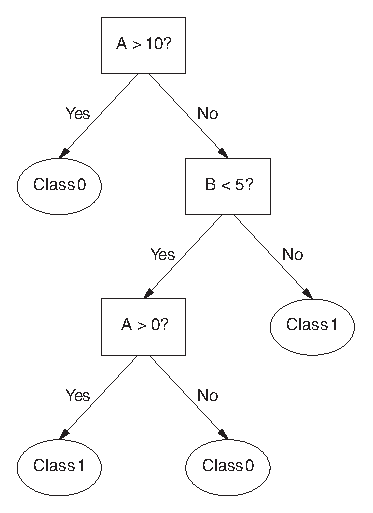
\includegraphics{img/dectree}}
  \caption{A very simple decision tree.}
  \label{fig:decisiontree}\vspace*{12pt}
\end{figure}

What I have described so far is the outline of the basic algorithm.
As with all greedy algorithms, there is no guarantee that it will find
the optimal solution, and therefore various heuristics play a large
role to ensure that the solution is as good as possible. Hence the
various published (and proprietary) algorithms for decision trees (you
may find references to CART, C4.5, and ID3) differ in such details
such as the following:
\begin{itemize}
\item What choice of purity/impurity measure is used?
\item At what level of purity does the splitting procedure stop?
  (Continuing to split a training set until all leaf nodes are entirely
  pure usually results in overfitting.)\pagebreak
\item Is the tree binary, or can a node have more than two children?
\item How should noncategorical attributes be treated? (For attributes
  that take on a continuum of values, we need to define the optimal
  splitting point.)
\item Is the tree postprocessed? (To reduce overfitting, some
  algorithms employ a pruning step that attempts to eliminate leaf
  nodes having too few elements.)
\end{itemize}

Decision trees are popular and combine several attractive features:
with good algorithms, decision trees are relatively cheap to build and
are always very fast to evaluate. They are also rather robust in the
presence of noise. It can even be instructive to examine the decision
points of a decision tree, because they frequently reveal interesting
information about the distribution of class labels (such as when 80
percent of the class information is contained in the topmost node).
However, algorithms for building decision trees are almost entirely
black-box and do not lend themselves to ad hoc modifications or
extensions.

There is an equivalence between decision trees and \emph{rule-based
  classifiers}. \index{rule-based classifiers} The latter consist of a set of rules (\ie, logical
conditions on attribute values) that, when taken in aggregate,
determine the class label of a test instance. There are two ways to
build a rule-based classifier. We can build a decision tree first and
then transform each complete path through the decision tree into a
single rule. Alternatively, we can build rule-based classifiers
directly from a training set by finding a subset of instances that can
be described by a simple rule. These instances are then removed from
the training set, and the process is repeated. (This amounts to a
bottom-up approach, whereas using a variant of Hunt's algorithm to
build a decision-tree follows a top-down approach.)

\index{decision trees|)}
\index{rule-based classifiers|)}  

\subsection{Other Classifiers}

In addition to the classifiers discussed so far, you will find others
mentioned in the literature. I'll name just two---mostly because of
their historical importance.

\emph{Fisher's linear discriminant analysis} (LDA)\index{Fisher's LDA (linear discriminant analysis)}\index{LDA (linear discriminant analysis)}\index{linear discriminant analysis (LDA)} was one of the
first classifiers developed. It is similar to principal component
analysis (see Chapter \ref{ch:reduction}). Whereas in PCA, we introduce
a new coordinate system to maximize  the spread along the new
coordinates axes, in LDA we introduce new coordinates to maximize the
separation between two classes that we try to distinguish. The
position of the means, calculated separately for each class, are taken
as the location of each class.

\emph{Artificial neural networks}\index{artificial neural networks}\index{neural networks, artificial} were conceived as extremely
simplified models for biological brains. The idea was to have a
network of nodes; each node receives input from several other nodes,
forms a weighted average of its input, and then sends it out to the
next layer of nodes.  During the learning stage, the weights used in
the weighted average are adjusted to minimize training error.  Neural
networks were very popular for a while but have recently fallen out
of favor somewhat. One reason is that the\vadjust{\pagebreak} calculations required are
more complicated than for other classifiers; another is that the whole
concept is very ad hoc and lacks a solid theoretical grounding.

\index{predictive analytics!algorithms for classification|)}
\index{algorithms, for classification|)}

 
% ============================================================
\section{The Process}

In addition to the primary algorithms for classification, various
techniques are important for dealing with practical problems. In this
section, we look at some standard methods commonly used to enhance
accuracy---especially for the important case when the most
``interesting'' type of class occurs much less frequently than the
other types. 


\subsection{Ensemble Methods: Bagging and Boosting}

\index{predictive analytics!ensemble methods}
\index{ensemble methods}  

The term \emph{ensemble methods} refers to a set of techniques for
improving accuracy by combining the results of individual or ``base''
classifiers. The rationale is the same as when performing some
experiment or measurement multiple times and then averaging the
results: as long as the experimental runs are independent, we can
expect that errors will cancel and that the average will be more
accurate than any individual trial. The same logic applies to
classification techniques: as long as the individual base classifiers
are independent, combining their results will lead to cancellation of
errors and the end result will have greater accuracy than the
individual contributions.

To generate a set of independent classifiers, we have to introduce
some randomness into the process by which they are built. We can
manipulate virtually any aspect of the overall system: we can play
with the selection of training instances (as in bagging and boosting),
with the selection of features (often in conjunction with random
forests), or with parameters that are specific to the type of
classifier used.

\emph{Bagging} \index{bagging} is an application of the bootstrap idea (see Chapter
\ref{ch:simulation}) to classification. We generate additional
training sets by sampling with replacement from the original training
set. Each of these training sets is then used to train a separate
classifier instance. During production, we let each of these instances
provide a separate assessment for each item we want to classify. The
final class label is then assigned based on a majority vote or similar
technique.

\emph{Boosting} \index{boosting} is another technique to generate additional training
sets using a bootstrap approach. In contrast to bagging, boosting is
an iterative process that assigns higher weights to instances
misclassified in previous rounds.  As the iteration progresses, higher
emphasis is placed on training instances that have proven hard to
classify correctly. The final result consists of the aggregate result
of all base classifiers generated during the iteration.  A popular
variant of this technique is known as ``AdaBoost.''

\emph{Random forests}\index{random forests}\index{decision trees} apply specifically to decision trees.  In this
technique, randomness is introduced not by sampling from the training
set but by\vadjust{\pagebreak} randomly choosing what features to use when building the
decision tree. Instead of examining all features at every node to find
the feature that gives the greatest gain ratio, only a subset of
features is evaluated for each tree.

\spreadlong{-13pt}

\subsection{Estimating Prediction Error}

\index{predictive analytics!prediction error}
 
Earlier, we already talked about the difference between the training
and the generalization error: \index{training errors} the training error is the final error
rate that the classifier achieves on the training set. It is usually
not a good measure for the accuracy of the classifier on \emph{new}
data (\ie, on data that was not used to train the classifier). For
this reason, we hold some of the data back during training, and use it
later as a test set. The error that the classifier achieves on this test
set is a much better measure for the generalization error that we can
expect when using the classifier on entirely new data.

If the original data set is very large, there is no problem in
splitting it into a training and a test set. In reality, however,
available data sets are always ``too small,'' so that we need to make
sure we use the available data most efficiently, using a process known
as \emph{cross-validation}. \index{cross-validation} 

The basic idea is that we randomly divide the original data set into
$k$ equally sized chunks. We then perform $k$ training and test runs.
In each run, we omit one of the chunks from the training set and
instead use it as the test set. Finally, we average the generalization
errors from all $k$ runs to obtain the overall expected generalization
error.

A value of $k=10$ is typical, but you can also use a value like $k=3$.
Setting $k=n$, where $n$ is the number of available data points, is
special: in this so-called ``leave-one-out'' cross-validation, we
train the classifier on all data points except one and then try to
predict the omitted data point---this procedure is then repeated for
all data points. (This prescription is similar to the jackknife
process that was mentioned briefly in Chapter \ref{ch:simulation}.)

Yet another method uses the idea of random sampling \emph{with
  replacement}, which is characteristic of bootstrap techniques (see
Chapter \ref{ch:simulation}). Instead of dividing the available data
into $k$ nonoverlapping chunks, we generate a bootstrap sample by
drawing $n$ data points with replacement from the\vadjust{} original $n$ data
points. This bootstrap sample will contain some of the data points
more than once,  and some not at all: overall, the fraction of the
unique data points included in the bootstrap sample will be about
$1-e^{-1} \approx 0.632$ of the available data points---for this
reason, the method is often known as the \emph{0.632 bootstrap}.  The
bootstrap sample is used for training, and the data points not
included in the bootstrap sample become the test set. This process can
be repeated several times, and the results averaged as for
cross-validation, to obtain the final estimate for the generalization
error.

(By the way, this is basically the ``unique visitor'' problem that we
discussed in Chapters \ref{ch:probability} and
\ref{ch:simulation}---after $n$ days (draws) with one random visitor
each day (one data point selected per draw), we will have seen
$1-e^{-\frac{1}{n}n} = 1-e^{-1}$ unique visitors (unique data points).)


\subsection{Class Imbalance Problems}

\index{predictive analytics!class imbalance problems}
\index{class imbalance problems} 

A special case of particular importance concerns situations where one
of the classes occurs much less frequently than any of the other
classes in the data set---and, as luck would have it, that's usually
the class we are interested in! Consider credit card fraud detection,
for instance: only one of every hundred credit card transactions may
be fraudulent, but those are exactly the ones we are interested in.
Screening lab results for patients with elevated heart attack risk or
inspecting manufactured items for defects falls into the same camp:
the ``interesting'' cases are rare, perhaps extremely rare, but those
are precisely the cases that we want to identify.

For cases like this, there is some additional terminology as well as
some special techniques for overcoming the technical difficulties.
Because there is one particular class that is of greater interest, we
refer to an instance belonging to this class as a \emph{positive
  event} and the class itself as the \emph{positive class}. With this
terminology, entries in the confusion matrix (see Table
\ref{tbl:confusion}) are often referred to as true (or false)
positives (or negatives).

I have always found this terminology very confusing, in part because
what is called ``positive'' is usually something \emph{bad}: a
fraudulent transaction, a defective item, a bad heart.~Table
\ref{tbl:confusioncheat} shows a confusion matrix employing the
special terminology for problems with a class imbalance---and also an
alternative terminology that may be more intuitive.

\begin{table}
\def\vrl{\smash{\vrule height38.7pt width.25pt depth3pt}}%
\tabcolsep11pt\tbl{Terminology for the confusion matrix in the case of class 
  imbalance (\ie ``bad'' outcomes are much less frequent than 
  ``good'' outcomes)\label{tbl:confusioncheat}}{%
\begin{tabular}{l@{\hskip9pt}c@{\hskip9pt}l@{\hskip9pt}c@{\hskip9pt}l}\toprule
 & & \TCH{Predicted:  {\itshape Bad}} && \TCH{Predicted: \textit{Good}} \\\colrule
\TCH{Actually: {\itshape Bad}}   && True positive: ``Hit''  && False negative: ``Miss'' \\\colrule
\TCH{Actually: {\itshape Good}}  &\vrl & False positive: ``False alarm'' &\vrl & True negative: ``Correct rejection'' \\
\end{tabular}}\vspace*{-9pt}
\end{table}

The two different types of errors may have very different costs
associated with them.  From the point of view of a merchant accepting
credit cards as payment, a false negative (\ie, a fraudulent
transaction incorrectly classified as ``not fraudulent''---a ``miss'')
results in the total loss of the  item purchased, whereas a false
positive (a valid transaction incorrectly classified as ``not
valid''---a ``false alarm'') results only in the loss of the profit
margin on that item.

The usual metrics by which we evaluate a classifier (such as accuracy
and error rate), may not be very meaningful in situations with pronounced
class imbalances: keep in mind that the trivial classifier that
labels \emph{every} credit card transaction as ``valid'' is 99 percent
accurate---and entirely useless! Two metrics that provide better
insight into the ability of a classifier to detect instances belonging
to the positive class are \emph{recall} \index{recall} and \emph{precision}. \index{precision!metrics} The
precision is the fraction of correct\vadjust{\pagebreak} classifications among all
instances labeled positive; the recall is the fraction of correct
classifications among all instances labeled negative: 
\begin{align*}
\text{precision} & 
= \frac{\text{true positives}}{\text{true positives}+\text{false positives}} \\
\text{recall} & 
= \frac{\text{true positives}}{\text{true positives}+\text{false negatives}}
\end{align*}

You can see that we will need to strike a balance. On the one hand, we
can build a classifier that is very aggressive, labeling many
transactions as ``bad,'' but it will have a high false-positive rate,
and therefore low precision. On the other hand, we can build a
classifier that is highly selective, marking only those instances that
are blatantly fraudulent as ``bad,'' but it will have a high rate of
false negatives and therefore low recall. These two competing goals
(to have few false positives and few false negatives) can be
summarized in a graph known as a \emph{receiver operating
  characteristic} (ROC) curve. \index{ROC (receiver operating characteristic) curve} (The concept originated in signal
processing, where it was used to describe the ability of a receiver to
distinguish a true signal from a spurious one in the presence of
noise, hence the name.)

\begin{figure}
\centerline{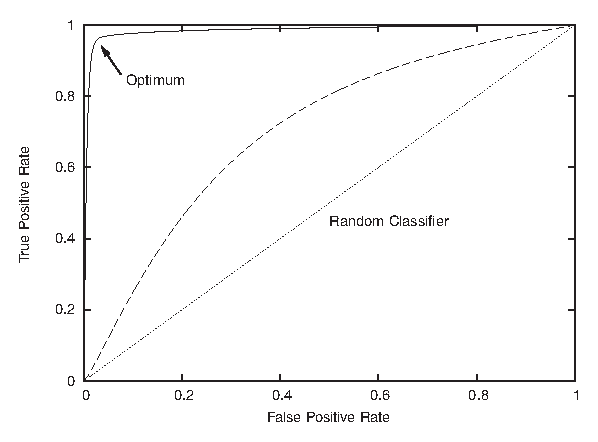
\includegraphics{img/roc}}
  \caption{A ROC (receiver operating characteristic) curve: the
    trade-off between true positives (``hits'') and false positives
    (``false alarms''), for three different classifier
    implementations.}
  \label{fig:roc}\vspace*{-6pt}
\end{figure}

Figure \ref{fig:roc} shows an example of a ROC curve. Along the
horizontal axis, we plot the false positive rate (good events that were
labeled as bad---``false alarms'') and along the vertical axis we plot
the true positive rate (bad events labeled as bad---``hits'').  The
lower-left corner corresponds to a maximally conservative classifier,
which labels every instance as good; the upper-right corner
corresponds to a maximally aggressive classifier, which labels
everything as bad. We can now imagine tuning the parameters and
thresholds of our classifier to shift the balance between ``misses''
and ``false alarms'' and thereby mapping out the characteristic curve
for our classifier.\vadjust{\pagebreak}  The curve for a random classifier (which assigns
a positive class label with fixed probability $p$, irrespective of
attribute values) will be close to the diagonal: it is equally likely
to classify a good instance as good as it is to classify a bad one as
good, hence its false positive rate equals its true positive rate. In
contrast, the ideal classifier would have a true positive rate equal
to 1 throughout.  We want to tune our classifier so that it
approximates the ideal classifier as nearly as possible.

Class imbalances pose some technical issues during the training phase:
if positive instances are extremely rare, then we want to make sure to
retain as much of their information as possible in the training set.
One way to achieve this is by oversampling (\ie, resampling) from the
positive class instances---and undersampling from the negative class
instances---when generating a training set. 

% ============================================================
\section{The Secret Sauce}

\index{predictive analytics!issues}
 
All this detail about different algorithms and processes can easily
leave the impression that that's all there is to classification. That
would be unfortunate, because it leaves out what can be the most
important but also the most difficult part of the puzzle: finding the
right attributes!

The choice of attributes matters for successful
classification---arguably more so than the choice of classification
algorithm.  Here is an interesting case story. Paul Graham has written
two essays on using Bayesian classifiers for spam
filtering.\footnote{``A Plan for Spam''
  (\url{http://www.paulgraham.com/spam.html}) and ``Better Bayesian
  Filtering''\\ (\url{http://www.paulgraham.com/better.html}).} In the
second one, he describes how using the information contained in the
email \emph{headers} is critical to obtaining good classification
results, whereas using only information in the \emph{body} is not
enough. The punch line here is clear: in practice, it matters a lot
which features or attributes you choose to include.

Unfortunately, when compared with the extremely detailed information
available on different classifier algorithms and their theoretical
properties, it is much more difficult to find good guidance regarding
how best to choose, prepare, and encode features for classification.
(None of the current books on classification discuss this topic at
all.)

I think there are several reasons for this relative lack of easily
available information---\break despite the importance of the topic. One of
them is lack of rigor: whereas one can prove rigorous theorems on
classification algorithms, most recommendations for feature
preparation and encoding would necessarily be empirical and heuristic.
Furthermore, every problem domain is different, which makes it
difficult to come up with recommendations that would be applicable
more generally. The implication is that factors such as experience,
familiarity with the problem domain, and lots of time-consuming trial
and error are essential when\vadjust{\pagebreak} choosing attributes for
classification.  (A last reason for the relative lack of available
information on this topic may be that some prefer to keep their cards
a little closer to their chest: they may tell you how it works ``in
theory,'' but they won't reveal all the tricks of the trade necessary
to fully replicate the results.)

The difficulty of developing some recommendations that work in general
and for a broad range of application domains may also explain one
particular observation regarding classification:
% I am referring to 
the apparent scarcity of spectacular, well-publicized successes.  Spam
filtering seems to be about the only application that clearly works
and affects many people directly.  Credit card fraud detection and
credit scoring are two other widely used (if less directly visible)
applications. But beyond those two, I see only a host of smaller,
specialized applications. This suggests again that every successful
classifier implementation depends strongly on the details of the
particular problem---probably more so than on the choice of algorithm.

% It also flies in the face of the ``data mining'' philosophy, of
% crunching numbers until something meaningful comes out.

\spreadlong{-13pt}
% ============================================================
\section{The Nature of Statistical Learning}

\index{predictive analytics!statistical learning|(}
 
Now that we have seen some of the most commonly used algorithms for
classification as well as some of the related practical techniques,
it's easy to feel a bit overwhelmed---there seem to be so many
different approaches (each nontrivial in its own way) that it can be
hard to see the commonalities among them: the ``big picture'' is
easily lost. So let's step back for a moment and reflect on the
specific challenges posed by classification problems and on the
overall strategy by which the various algorithms overcome these
challenges.

% \subsection{The Nature of the Problem}

The crucial problem is that from the outset, we don't have good insight
into which features are the most relevant in predicting the class---in
fact, we may have no idea at all about the processes (if any!) that
link observable features to the resulting class. Because we don't know
ahead of time which features are likely to be most important, we need
to retain them all and perhaps even expand the feature set in an
attempt to include any possible clue we can get. In this way, the
problem quickly becomes very multi-dimensional. That's the first
challenge.

But now we run into a problem: multi-dimensional data sets are
invariably \emph{sparse} data sets. Think of a histogram with (say) 5
bins per dimension. In one dimension, we have 5 bins total. If we want
on average at least 5 items per bin, we can make do with 25 items
total. Now consider the same data  set in two dimensions. If we still
require 5 bins per dimension, we have a total of 25 bins, so that each
bin contains on average only a single element. But it is in three
dimensions that the situation becomes truly dramatic: now there are
125 bins, so we can be sure that the majority of bins will contain
\emph{no} element at all! It gets even worse in higher dimensions.
(Mathematically speaking, the problem is that the number of bins grows
exponentially with the number of dimensions: $N^d$, where $d$ is the
number of dimensions and $N$ is the number of bins per dimension. No
matter what you do, the number of cells is going to grow faster than
you can obtain data.  This problem is known as the \emph{curse of
  dimensionality}.)\index{curse of dimensionality}\index{dimensionality, curse of} That's the second challenge.

It is this combinatorial explosion that drives the need for larger and
larger data sets. We have just seen that the the number of possible
attribute value combinations grows exponentially; therefore, if we
want to have a reasonable chance of finding at least one instance of
each possible combination in our training data, we need to have very
large data sets indeed. Yet despite our best efforts, we will
frequently end up with a sparse data set (as discussed above).
Nevertheless, we will often deal with inconveniently large data sets.
That's the third challenge.

% \subsection{The Nature of the Solution}

Basically all classification algorithms deal with these challenges by
using some form of \emph{interpolation} between points in the sparse
data set. In other words, they attempt to smoothly fill the gaps left
in the high-dimensional feature space, supported only by a
(necessarily sparse) set of points (\ie, the training instances).

Different algorithms do this in different ways: nearest-neighbor
methods and naive Bayesian classifiers explicitly ``smear out'' the
training instances to fill the gaps locally, whereas regression and
support vector classifiers construct global structures to form a
smooth decision boundary from the sparse set of supporting points.
Decision trees are similar to nearest-neighbor methods in this regard
but provide a particularly fast and efficient lookup of the most
relevant neighbors.  Their differences aside, all algorithms aim~to
fill the gaps between the existing data points in some smooth,
consistent way.

% We assume that we understand the system so well that we have reason to 
% believe that ``past performance is a good indicator of future results''. 

% Understanding-free learning

This brings us to the question of what can actually be predicted in
this fashion.  Obviously, class labels must depend on attribute
values, and they should do so in some smooth, predictable fashion.  If
the relationship between attribute values and class labels is too
crazy, no classifier will be very useful.

Furthermore, the distribution of attribute values for different
classes must \emph{differ}, for otherwise no classifier will be able
to distinguish classes by examining the attribute\break values.

Unfortunately, there is---to my knowledge---no independent, rigorous
way of determining whether the information contained in a data set is
sufficient to allow the data to be classified. To find out, we must
build an actual classifier. If it works, then obviously there
\emph{is} enough information in the data set for classification. But
if it does \emph{not} work, we have learned nothing, because it is
always possible that a different or more sophisticated classifier
\emph{would} work. But without an independent test, we can spend an
infinite amount of time building and refining classifiers on data sets
that contain no useful information. We encountered this kind of
difficulty already in Chapter \ref{ch:clustering} in the context of
clustering algorithms, but it strikes me as even more of a problem
here. The reason is that classification is by nature predictive (or at
least should be), whereas uncertainty of this sort seems more
acceptable in an exploratory technique such as clustering.

To make this more clear, suppose we have a large, rich data set: many
records with many features. We then arbitrarily assign class labels A
and B to the records in the data set.  Now, by construction, it is
clear that\vadjust{\pagebreak} there is no way to predict the labels from the
``data''---they are, after all, purely random! However, there is no
unambiguous  test that will clearly say so. We can calculate the
correlation coefficients between  each feature (or combination of
features) and the class label, we can look at the distribution of
feature values and see whether they differ from class to class, and so
eventually convince ourselves that we won't be able to build a good
classifier given this data set. But there is no clear test or
diagnostic that would give us, for instance, an upper bound on the
quality of any classifier that could be built based on this data set.
If we are not careful, we may spend a lot of time vainly attempting to
build a classifier capable of extracting useful information from this
data set. This kind of problem is a trap to be aware of!

% The absence of strong ``no-go theorems'' of this sort is a real
% handicap.

\index{predictive analytics!statistical learning|)}

\spreadlong{-13pt}

% ============================================================
\section{Workshop: Two Do-It-Yourself Classifiers}

\index{predictive analytics!two do-it-yourself classifiers|(}
 
With classification especially, it is really easy to end up with a
black-box solution: a tool or~library that provides an implementation
of a classification algorithm---but one that we~would not be able to write
ourselves if we had to.  This kind of situation always makes~me~a bit
uncomfortable, especially if the algorithms require any parameter
tuning to work properly. In order to adjust such parameters
intelligently, I need to understand the~algorithm well enough that I
could at least provide a rough-cut version myself (much as I am happy
to rely on the library designer for the high-performance version).

In this spirit, instead of discussing an existing classification
library, I want to show you how to write straightforward (you might
say ``toy version'') implementations for two simple classifiers: a
nearest-neighbor lazy learner and a naive Bayesian classifier. (I'll
give some pointers to other libraries near end of the section.)

We will test our implementations on \emph{the} classic data set in all
of classification: Fisher's Iris data set.\index{Fisher's Iris data set}\footnote{First published in 1936. The data set is available from many 
  sources, for example in the ``Iris'' data set on the UCI Machine 
  Learning repository at \url{http://archive.ics.uci.edu/ml/}.} The data set
contains measurements of four different parts of an iris flower (sepal
length and width, petal length and width). There are 150 records in
the data set, distributed equally among three species of Iris
(\emph{Iris setosa}, \emph{versicolor}, and \emph{virginica}). The
task is to predict the species based on a given a set of measurements.

First of all, let's take a quick look at the distributions of the four
quantities, to see whether it seems feasible to distinguish the three
classes this way. Figure \ref{fig:predhistos} shows histograms
(actually, kernel density estimates) for all four quantities,
separately for the three classes. One of the features (sepal width)
does not seem very promising, but the distributions of the other three
features seem sufficiently separated that it should be possible to
obtain good classification\vadjust{\pagebreak} results.

\begin{figure}
\centerline{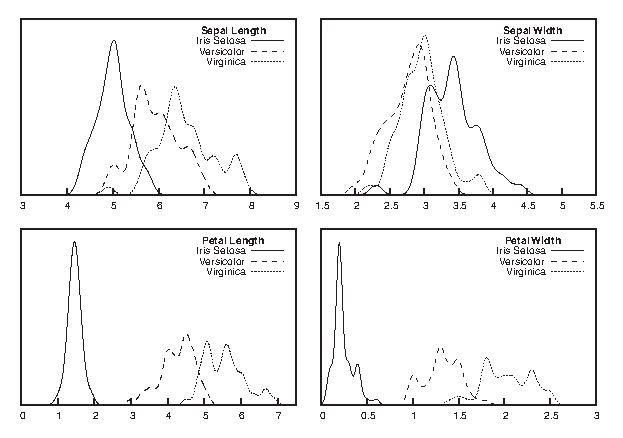
\includegraphics{img/predhistos}}
  \caption{The distribution of the four attributes in the Iris data
    set, displayed separately for the three classes.}
  \label{fig:predhistos}
\end{figure}

As preparation, I split the original data set into two parts: a
training set (in the file \texttt{iris.trn}) and a test set (in file
\texttt{iris.tst}). I randomly  selected five records from each class
for the test set; the remaining records were used for training.  The
test set is shown in full~below: the columns are  (in order) sepal
length, sepal width, petal length, petal width,~and the class label.
(All measurements are in centimeters and to millimeter precision.)\vspace*{13pt}

\begin{verbatim}
5.0,3.6,1.4,0.2,Iris-setosa
4.8,3.0,1.4,0.1,Iris-setosa
5.2,3.5,1.5,0.2,Iris-setosa
5.1,3.8,1.6,0.2,Iris-setosa
5.3,3.7,1.5,0.2,Iris-setosa
5.7,2.8,4.5,1.3,Iris-versicolor
5.2,2.7,3.9,1.4,Iris-versicolor
6.1,2.9,4.7,1.4,Iris-versicolor
6.1,2.8,4.7,1.2,Iris-versicolor
6.0,3.4,4.5,1.6,Iris-versicolor
6.3,2.9,5.6,1.8,Iris-virginica
6.2,2.8,4.8,1.8,Iris-virginica
7.9,3.8,6.4,2.0,Iris-virginica
5.8,2.7,5.1,1.9,Iris-virginica
6.5,3.0,5.2,2.0,Iris-virginica
\end{verbatim}\vspace*{3pt}

Our implementation of the nearest-neighbor classifier is shown in the
next listing. The implementation is exceedingly simple---especially
once you realize that about two thirds of the listing deal with file
input and output. The\vadjust{\pagebreak} actual ``classification'' is a matter of three
lines in the middle:

\begin{verbatim}
# A Nearest-Neighbor Classifier

from numpy import *

train = loadtxt( "iris.trn", delimiter=',', usecols=(0,1,2,3) )
trainlabel = loadtxt( "iris.trn", delimiter=',', usecols=(4,), dtype=str )

test = loadtxt( "iris.tst", delimiter=',', usecols=(0,1,2,3) )
testlabel = loadtxt( "iris.tst", delimiter=',', usecols=(4,), dtype=str )

hit, miss = 0, 0
for i in range( test.shape[0] ):
    dist = sqrt( sum( (test[i] - train)**2, axis=1 ) )
    k = argmin( dist )

    if trainlabel[k] == testlabel[i]:
        flag = '+'
        hit += 1
    else:
        flag = '-'
        miss += 1
        
    print flag, "\t Predicted: ", trainlabel[k], "\t True: ", testlabel[i]

print
print hit, "out of", hit+miss, "correct - Accuracy: ", hit/(hit+miss+0.0)
\end{verbatim}

The algorithm loads both the training and the test data set into
two-dimensional NumPy arrays. Because all elements in a NumPy array
must be of the same type, we store the class labels (which are
strings, not numbers) in separate vectors.

Now follows the actual classification step: for each element of the
test set, we calculate the Euclidean distance to each element in the
training set. We make use of NumPy ``broadcasting'' (see the Workshop
in Chapter \ref{ch:univariate}) to calculate the distance of the test
instance \texttt{test[i]} from \emph{all} training instances in one
fell swoop. (The argument \texttt{axis=1} is necessary to tell NumPy
that the sum in the Euclidean distance should be taken over the
\emph{inner} (horizontal) dimension of the two-dimensional array.)
Next, we use the \texttt{argmin()} function to obtain the index of the
training record that has the smallest distance to the current test
record: this is our predicted class label. (Notice that we base our
result only on a single record---namely the closest training
instance.)

Simple as it is, the classifier works very well (on this data set).
For the test set shown, all records in the test set are classified
correctly!

The naive Bayesian classifier implementation is next. A naive Bayesian
classifier needs an estimate of the probability distribution $P(
\text{class $C$} \, | \, \text{feature $x$} )$,  which we find from a
histogram of attribute values, separately for each class. In this
case, we need a total of 12 histograms (3 classes $\times$ 4
features). I maintain this data in a triply nested data structure:
\texttt{histo[label][feature][value]}.  The first index is the class
label, the\vadjust{\pagebreak} second index specifies the feature, and the third contains
the values of the feature that occur in the histogram. The value
stored in the histogram is the number of times that each value has
been observed:  \leaflong{18pt}
% I use this kind of nested histogram data structure all the time.

\begin{verbatim}
# A Naive Bayesian Classifier

total = \{\}  # Training instances per class label
histo = \{\}  # Histogram

# Read the training set and build up a histogram
train = open( "iris.trn" )
for line in train:
    # seplen, sepwid, petlen, petwid, label
    f = line.rstrip().split( ',' )
    label = f.pop()

    if not total.has_key( label ):
        total[ label ] = 0
        histo[ label ] = [ \{\}, \{\}, \{\}, \{\} ]

    # Count training instances for the current label
    total[label] += 1

    # Iterate over features
    for i in range( 4 ):
        histo[label][i][f[i]] = 1 + histo[label][i].get( f[i], 0.0 )
        
train.close()

# Read the test set and evaluate the probabilities
hit, miss = 0, 0
test = open( "iris.tst" )
for line in test:
    f = line.rstrip().split( ',' )
    true = f.pop()

    p = \{\} # Probability for class label, given the test features
    for label in total.keys():
        p[label] = 1
        for i in range( 4 ):
            p[label] *= histo[label][i].get(f[i],0.0)/total[label]

    # Find the label with the largest probability
    mx, predicted = 0, -1
    for k in p.keys():
        if p[k] >= mx:
            mx, predicted = p[k], k

    if true == predicted:
        flag = '+'
        hit += 1

    else:
        flag = '-'
        miss += 1
 \end{verbatim}

\begin{verbatim}       
    print flag, "\t", true, "\t", predicted, "\t",
    for label in p.keys():
        print label, ":", p[label], "\t",
    print

print
print hit, "out of", hit+miss, "correct - Accuracy: ", hit/(hit+miss+0.0)

test.close()
\end{verbatim}

\looseness-1I'd like to point out two implementation details.  The first is that
the second index is an integer, which I use instead of the feature
names; this simplifies some of the loops in the program. The second
detail is more important: I know that the feature values are given in
centimeters, with exactly one digit after the decimal point. In other
words, the values are already discretized, and so I don't need to
``bin'' them any further---in effect, each bin in the histogram is one
millimeter wide.  Because I never need to operate on the feature
values, I don't even convert them to numbers: I read them as strings
from file and use them (as strings) as keys in the histogram. Of
course, if we wanted to use a different bin width, then we would have
to convert them into numerical values so that we can operate on them.

In the evaluation part, the program reads data points from the test
set and then evaluates the probability that the record belongs to a
certain class for all three class labels. We then pick the class label
that has the highest probability. (Notice that we don't need an
explicit factor for the prior probability, since we know that each
class is equally likely.)

\looseness-1On the test set shown earlier, the Bayesian classifier does a little
worse than the nearest neighbor classifier: it correctly classifies 12
of 15 instances for a total accuracy of 80 percent.

If you look at the results of the classifier more closely, you will
immediately notice a couple of problems that are common with Bayesian
classifiers. First of all, the posterior probabilities are
\emph{small}.  This should come as no surprise: each Bayes factor is
smaller than $1$ (because it's a probability), so their product
becomes very small very quickly. To avoid underflows, it's usually a
good idea to add the logarithms of the probabilities instead of
multiplying the probabilities directly. In fact, if you have a greater
number of features, this becomes a necessity. The second problem is
that many of the posterior probabilities come out as exactly zero:
this occurs whenever no entry in the histogram can be found for at
least one of the feature values in the test record; in this case the
histogram evaluates to zero, which means the entire product of
probabilities is also identical to zero. There are different ways of
dealing with this problem---in our case, you might want to experiment
with replacing the histogram of discrete feature values with a kernel
density estimate (similar to those in Figure \ref{fig:predhistos}),
which, by construction, is nonzero everywhere. Keep in mind that you will need to
determine a suitable bandwidth for each histogram!

Let me be clear: the implementations of both classifiers are extremely
simpleminded. My intention here is to demonstrate the basic ideas
behind these algorithms in as few lines of code as possible---and also
to show that there is nothing mystical about writing a simple
classifier. Because the implementations are so simple, it is easy to
continue experimenting\vadjust{\pagebreak} with them: can we do better if we use a larger
number of neighbors in our nearest-\break neighbor classifier?  How about a
different distance function? In the naive Bayesian classifier, we can
experiment with different bin widths in the histogram or, better yet,
replace the histogram of discrete bins with a kernel density estimate.
In either case, we need to start thinking about runtime efficiency:
for a data set of only 150 elements this does not matter much, but
evaluating a kernel density estimate of a few thousand points can be
quite expensive!

If you want to use an established tool or library, there are several
choices in the open source world. Three projects have put together
entire data analysis and mining ``toolboxes,'' complete with graphical
user interface, plotting capabilities, and various plug-ins:
RapidMiner (\url{http://rapid-i.com/}) and WEKA
(\url{http://www.cs.waikato.ac.nz/ml/} \url{weka/}), which are both in Java
as well as Orange (\url{http://www.ailab.si/orange/}), which is in
Python. WEKA has been around for a long time and is very well
established; RapidMiner is part of a more comprehensive tool suite
(and includes WEKA as a plug-in). Orange is an alternative using
Python.

All three of these projects use a ``pipeline'' metaphor: you select
different processing steps (discretizers, smoothers, principal
component analysis, regression, classifiers) from a toolbox and
string them together to build up the whole analysis workflow entirely
within the tool.  Give it a shot---the idea has a lot of appeal, but
I must confess that I have \emph{never} succeeded in doing anything
nontrivial with any of them!

There are some additional libraries worth checking out that have
Python interfaces: libSVM
(\url{http://www.csie.ntu.edu.tw/~cjlin/libsvm/}) and Shogun
(\url{http://www.shogun-toolbox}\break \url{.org/}) provide implementations of
support vector machines, while the Modular toolkit for Data Processing
(\url{http://mdp-toolkit.sourceforge.net/}) is more general. (The
latter also adheres to the ``pipeline'' metaphor.)

Finally, all classification algorithms are also available as R
packages. I'll mention just three: the \texttt{class} package for
nearest-neighbor classifiers and the \texttt{rpart} package for
decision trees (both part of the R standard distribution) as well as
the \texttt{e1071} package (which can be found on CRAN) for support
vector machines and naive Bayesian classifiers.

\index{predictive analytics!two do-it-yourself classifiers|)}


\vspace*{-6pt}
% ============================================================
\section{Further Reading}
\begin{itemize}
\item \cit{Introduction to Data Mining}{Pang-Ning Tan, Michael
    Steinbach, and Vipin Kumar}{Addison-Wesley}{2005}
  This is my favorite book on data mining. It contains two accessible
  chapters on classification.

\item \cit{The Elements of Statistical Learning}{Trevor Hastie, Robert
    Tibshirani, and Jerome Friedman}{2nd ed., Springer}{2009}

  This book exemplifies some of the problems with current
  machine-learning theory: an entire book of highly nontrivial
  mathematics---and what feels like not a single real-world example or
  discussion of ``what to use when.''
%\item \cit{Introduction to Data Mining}{Pang-Ning Tan et al}{Addison-Wesley}{2005}
%  This is my favorite book on data mining. It contains two accessible
%  chapters on classification.
%
%%, Michael
%%    Steinbach, and Vipin Kumar
%
%\item \cit{The Elements of Statistical Learning}{Trevor Hastie et al}{2nd ed., Springer}{2009}
%
%  This book exemplifies some of the problems with current
%  machine-learning theory: an entire book of highly nontrivial
%  mathematics---and what feels like not a single real-world example or
%  discussion of ``what to use when.''
\end{itemize}
\index{data analysis!predictive analytics|)} 
\index{predictive analytics|)} 
\clearpage
\
\thispagestyle{empty}
\
\clearpage